\documentclass{article}
\usepackage{geometry}
\geometry{a4paper, portrait, margin=1.5in}

\usepackage{hyperref}
\hypersetup{
    colorlinks=true,
    linkcolor=black,
    filecolor=magenta,
    urlcolor=blue,
}

\usepackage{graphicx}
\graphicspath{ {images/} }

\usepackage{tcolorbox}
\usepackage{textcomp}
\usepackage{gensymb}
\usepackage{indentfirst}

\title{RJ Electrical Training Week 3 Guide}
\author{Alex Xu}
\begin{document}
\maketitle{}
\setcounter{tocdepth}{2}
\tableofcontents
\pagebreak

\section{Introduction}
In last week's training, we used Arduino and some separate supporting electrical components to control motors. They exist independently from each other and is cumbersome if they're installed on the robot as in their current state. A PCB that integrates all the components would be a lot more manageable when installed on a robot. That is the eventual goal of this training. \par
In this week, we will be \textbf{prototyping the PCB by replicating it on a breadboard} so we can verify that the circuit works. \textbf{\emph{Important steps need to be taken are highlighted in bold italic font.}}

\begin{figure}[!h]
    \center
    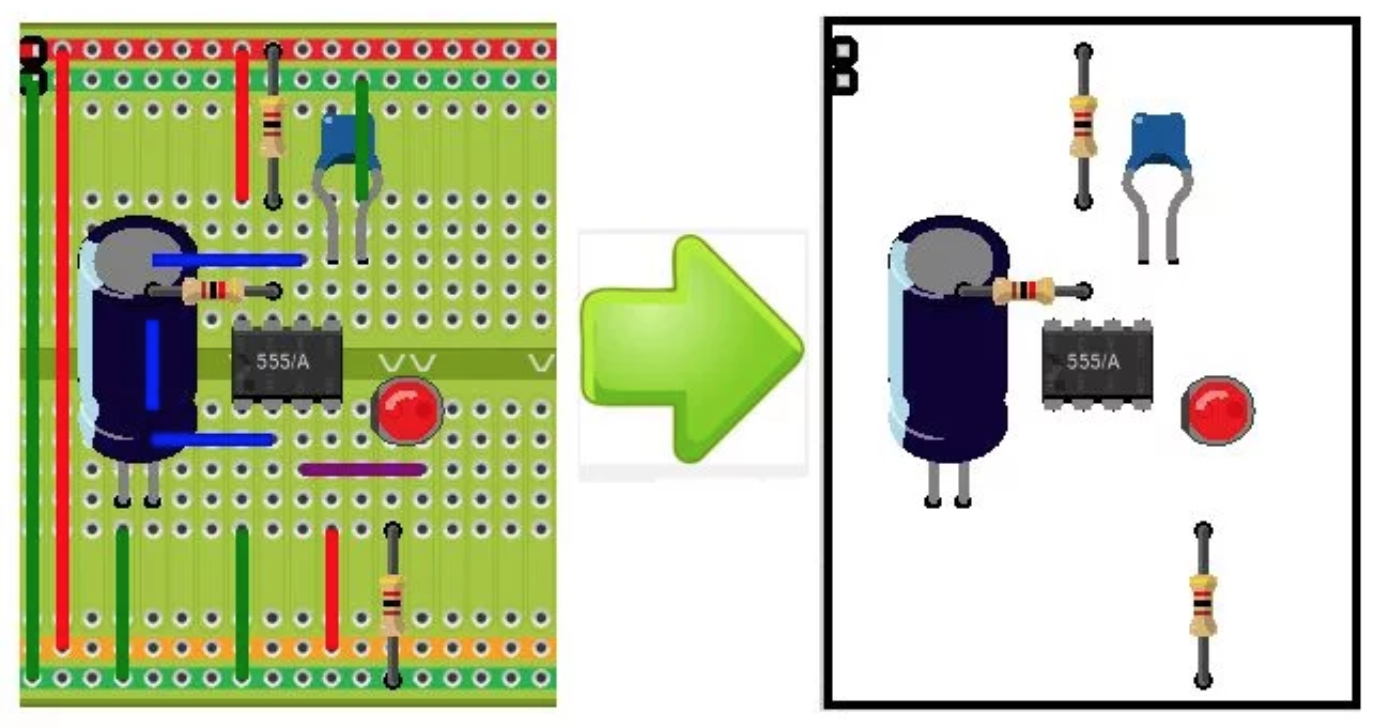
\includegraphics[width=0.6\textwidth,height=0.6\textheight,keepaspectratio]{breadboard_to_pcb}
\end{figure}

\section{IC Packages}
``The package is what encapsulates the integrated circuit die and splays it out into a device we can more easily connect to. ... There are many different types of packages, each of which has unique dimensions, mounting-types, and/or pin-counts.''  - SparkFun. \par
All packages can be divided by their mounting types: through-hole or surface-mount (SMD or SMT). Through-hole packages are generally bigger and much easier to work with. They're designed to be stuck through the holes on a board and soldered from the other side. They came exceptionally handy when used with a breadboard since they can be easily reconnected. SMD components are more commonly seen on PCBs.

\begin{figure}[!h]
    \center
    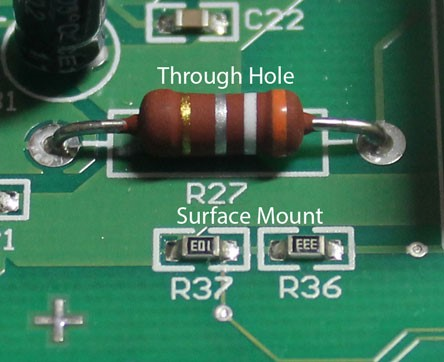
\includegraphics[width=0.4\textwidth,keepaspectratio]{throughvssmd}
    \caption {Through-Hole components vs SMD}
    \label{img:through_vs_smd}
\end{figure}

All of the packages to be used today will be through-hole components. Recall breadboard connections and prepare for . 

\begin{figure}[!h]
    \center
    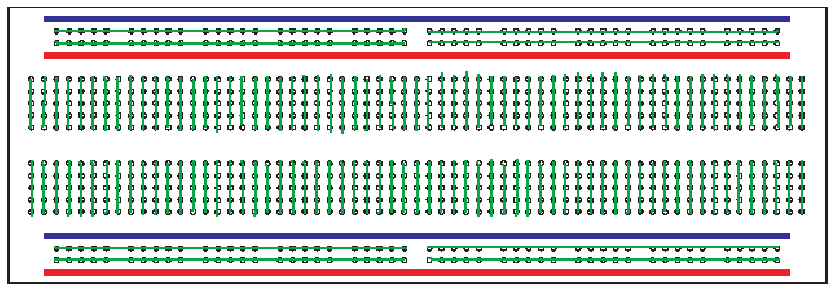
\includegraphics[width=0.8\textwidth,keepaspectratio]{Breadboard_Internal_Connections}
    \caption {Breadboard Internal Connections}
    \label{img:bread_connections}
\end{figure}



\section{Breadboarding}

\subsection{Placing the Important Chip}
\begin{table}[!h]
    \center
    \begin{tabular}{c|c|c}
        Name              & Quantity & Package   \\
        \hline
        ATMega328         & 1        & DIP      \\
        Linear Regulator & 1        & TO-220-3  \\
        Capacitor 0.33uF  & 1        & /       \\
        Capacitor 0.1uF   & 1        & /      \\
        Capacitor 22pF    & 2        & /        \\
        Battery Clip      & 1        & /        \\
        Crystal 16MHz     & 1        & /     
    \end{tabular}
    \caption{Component List for Trainii}
    \label{table:componentList}
\end{table}

Our board is rather simple and we would place our microcontroller(mcu) the \textbf{ATMega328} (See Table \ref{table:componentList}) first. \textbf{\emph{We place the ATMega328 component onto the breadboard}}. It is a Dual Inline Package (DIP), and DIP package need to be placed as shown in Figure \ref{img:dip_breadboard}. \par

\begin{tcolorbox} [title=Tips \& Tricks]
    \begin{itemize}
        \item % During breadboarding, we need to consider the sequence of putting components into the board. There are usually two types of components, the chips that does the work, and the peripheral components that support the important chips. The supporting components would cluster around the functioning chips. To avoid overcrowding the breadboard, it is usually suggested to place important chips first and afar from each other based on how much supporting components they have around them, then adding supporting components. \par
        \item Power rails does not need to have the same voltage across the entire breadboard and not all voltage lines need to go on power rails. 
    \end{itemize}
\end{tcolorbox}

\begin{figure}[!h]
    \center
    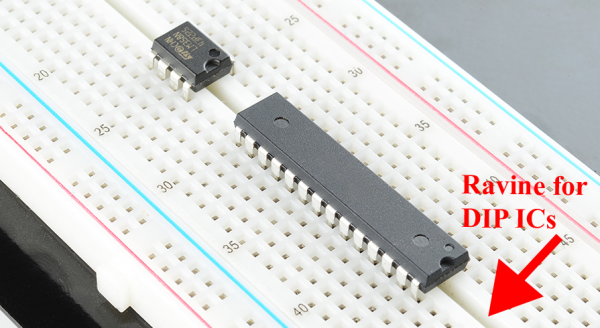
\includegraphics[width=0.4\textwidth,keepaspectratio]{dip_breadboard}
    \caption {Placing DIPs into breadboard}
    \label{img:dip_breadboard}
\end{figure}

\subsection{Adding Supporting Components}
The operation of our ATMega328 requires an external crystal. The operation of crystal requires 2 supporting capacitors. \textbf{\emph{Insert the crystal, 2 22pF capacitors onto the breadboard so it is equivalent to this schematics (Figure \ref{img:crystal}).}} GND means ground and refer to Figure \ref{img:bread_connections} for ground connection. Refer to the notch on one end of ATMega328 package and its datasheet for pin 9 and pin 10 location. \par

\begin{figure}[!h]
    \center
    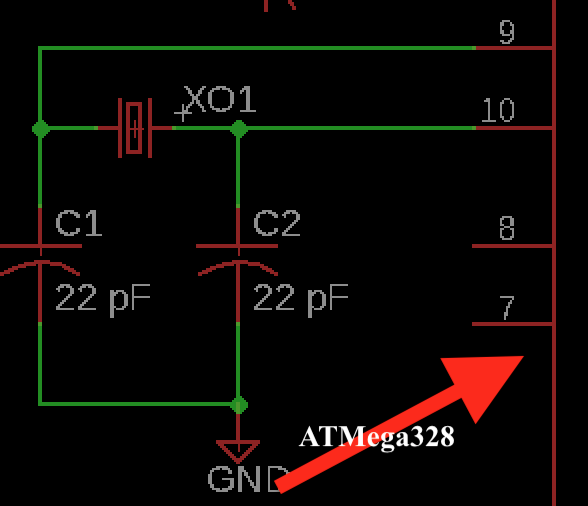
\includegraphics[width=0.4\textwidth,keepaspectratio]{crystal}
    \caption{Crystal Schematics}
    \label{img:crystal}
\end{figure}

ATMega328 also requires a decoupling capacitor to operate. \textbf{\emph{Connect a 0.1uF capacitor between the power and ground pin of ATMega.}}

\subsection{Adding Power Supply}
The next step would be the power supply. We want the ATMega mcu to run at 3.3V. However a 3.3V power supply is not very common therefore we will use a 9V battery and use a linear regulator to transform the voltage to 3.3V. \par
Connect the blue line of battery clip to the ground connection on breadboard. \emph{\textbf{Connect the linear regulator and 9V battery clip as shown in Figure \ref{img:linear_regulator}}}, $V_{in}$ corresponds to 9V and $V_{out}$ corresponds to 3.3V. Connect the power rail on the breadboard to the $V_{out}$ pin. 
% Capacitor value?

\begin{figure}[!h]
    \center
    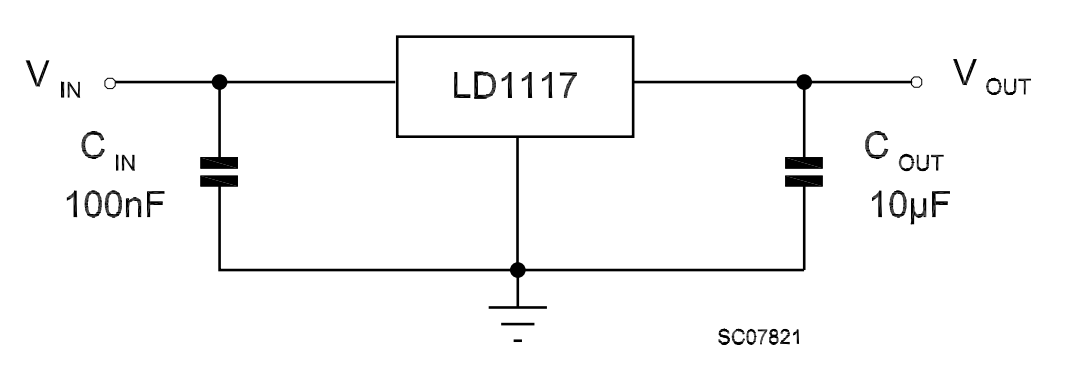
\includegraphics[width=0.8\textwidth,keepaspectratio]{linear_regulator}
    \caption{Power Circuit Schematics}
    \label{img:linear_regulator}
\end{figure}

\begin{tcolorbox} [title=Tips \& Tricks]
    \begin{itemize}
        \item Breadboard has multiple ground and power rails (red and blue). The ground need to be the same and stay 0V and different ground rails \textbf{will} have to be connected via jumper wire should you want to use them as ground.
        \item Power rails does not need to have the same voltage across the entire breadboard and not all voltage lines need to go on power rails. 
    \end{itemize}
\end{tcolorbox}

\subsection{Completing the Circuit}
\textbf{\emph{Connect all GND pins to ground rail, all VCC pins to power rail.}} Use a multimeter to test the continuity between power and ground rail to make sure it's not shorted. Check the board connection with the Figure \ref{img:egBBL}.

\begin{figure}[!h]
    \center
    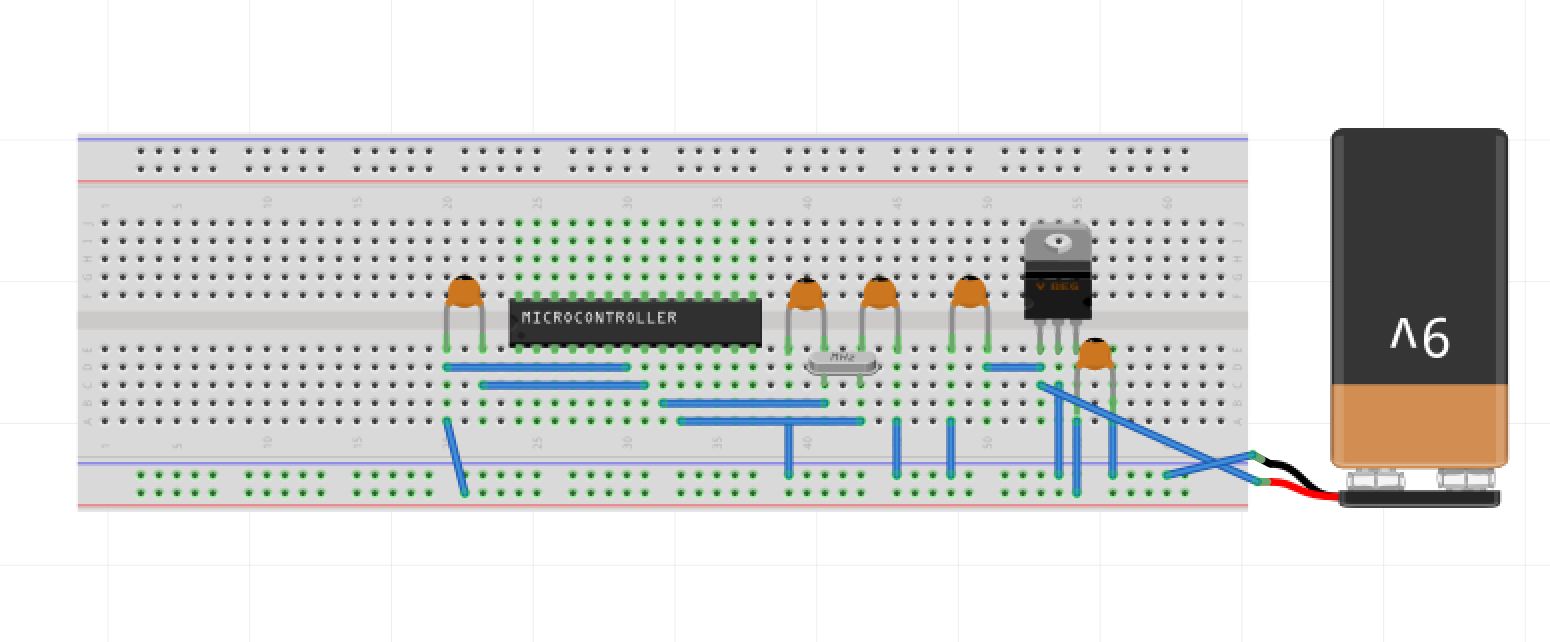
\includegraphics[width=0.8\textwidth,keepaspectratio]{egBBL}
    \caption{Example Breadboard Layout}
    \label{img:egBBL}
\end{figure}

\section{Using the Board}
Congratulations, you have just constructed a small-sized version of Arduino! Program the board to access its I/O pins and use it like an Arduino.
















\end{document}